\documentclass[12pt, landscape]{article}
\usepackage[scaled=0.92]{helvet}
\usepackage{multicol}
\usepackage{calc}
\usepackage{ifthen}
\usepackage[landscape]{geometry}
%\usepackage{hyperref}

\usepackage{newtxtext} 

%for strikeout
\usepackage{ulem}

%For editing parbox
\usepackage[table]{xcolor}
%For editing itemise margins, reduce iterm separaion and list separation
\usepackage{enumitem}
% For math
\usepackage{amsmath,amsthm,amsfonts,amssymb}

%For pictures / figures
\usepackage{color,graphicx,overpic}
\graphicspath{ {./images/} }

%\usepackage{newtxtext} 
%\usepackage{amssymb}
%\usepackage[table]{xcolor}
%\usepackage{vwcol}
%\usepackage{tikz}
%\usepackage{wrapfig}
%\usepackage{makecell}

\pdfinfo{
  /Title (IS2238.pdf)
  /Creator (Ger Teck)
  /Author (Ger Teck)
  /Subject ()
  /Keywords (tex)}

%% Margins for PAPER

% This sets page margins to .5 inch if using letter paper, and to 1cm
% if using A4 paper. (This probably isn't strictly necessary.)
% If using another size paper, use default 1cm margins.
\ifthenelse{\lengthtest { \paperwidth = 11in}}
	{ \geometry{top=.5in,left=.5in,right=.5in,bottom=.5in} }
	{\ifthenelse{ \lengthtest{ \paperwidth = 297mm}}
		{\geometry{top=1cm,left=1cm,right=1cm,bottom=1cm} }
		{\geometry{top=1cm,left=1cm,right=1cm,bottom=1cm} }
	}

% Turn off header and footer
\pagestyle{empty}

% for tight centres (less spacing)
\newenvironment{tightcenter}{%
  \setlength\topsep{0pt}
  \setlength\parskip{0pt}
  \begin{center}
}{%
  \end{center}
}

% Redefine section commands to use less space
\makeatletter
\renewcommand{\section}{\@startsection{section}{1}{0mm}%
                                {-1ex plus -.5ex minus -.2ex}%
                                {0.5ex plus .2ex}%x
                                {\normalfont\large\bfseries}}
\renewcommand{\subsection}{\@startsection{subsection}{2}{0mm}%
                                {-1explus -.5ex minus -.2ex}%
                                {0.5ex plus .2ex}%
                                {\normalfont\normalsize\bfseries}}
\renewcommand{\subsubsection}{\@startsection{subsubsection}{3}{0mm}%
                                {-1ex plus -.5ex minus -.2ex}%
                                {1ex plus .2ex}%
                                {\normalfont\small\bfseries}}
% change font
%\renewcommand{\familydefault}{\sfdefault}
%\renewcommand\rmdefault{\sfdefault}
\makeatother

% Define BibTeX command
\def\BibTeX{{\rm B\kern-.05em{\sc i\kern-.025em b}\kern-.08em
    T\kern-.1667em\lower.7ex\hbox{E}\kern-.125emX}}

% Don't print section numbers
\setcounter{secnumdepth}{0}

\setlength{\parindent}{0pt}
\setlength{\parskip}{0pt plus 0.5ex}

%% this changes all items (enumerate and itemize, reduce margins)
\setlength{\leftmargini}{0.5cm}
\setlength{\leftmarginii}{0.5cm}
\setlist[itemize,1]{leftmargin=2mm,labelindent=1mm,labelsep=1mm, itemsep = 1mm}
\setlist[itemize,2]{leftmargin=4mm,labelindent=1mm,labelsep=1mm, itemsep = 1mm}
\itemsep = 2mm
%\setlist{nosep}

% -------------------------------------------------------------------------------

% START OF DOCUMENT HERE

\begin{document}
\raggedright
\footnotesize
\begin{multicols*}{3}

% multicol parameters
% These lengths are set only within the two main columns
\setlength{\columnseprule}{0pt}
\setlength{\premulticols}{1pt}
\setlength{\postmulticols}{1pt}
\setlength{\multicolsep}{2pt}
\setlength{\columnsep}{2pt}

%% DOCUMENT NAME HERE
\begin{center}
     \Large{\textbf{IS2238 Economics of IT \& AI}} \\
\end{center}

% TABLE PACKAGE 
 \begin{center}
    \fbox{%
        \parbox{0.8\linewidth}{\centering \textcolor{black}{
            \\ \normalsize{AY22/23 Sem 2}}
            \\ {\footnotesize github.com/gerteck}
        }%
    }
  \end{center}

\section{1. Overview of Economics of IT}

\begin{itemize}
	\item \textbf{IT/AI are changing our lives, businesses, and economy.} Economics can provide a lens through which we can better understand this new economy and phenomena in a more systematic manner.
	\item High speed change in today’s digital age. (Digital revolution). Cause of change is computer \& comunications, technology such as integreted circuits, data speed and laptop capacity which have increased by many times. $\rightarrow$ Increase in employee productivity.
	\item \textbf{Moore’s Law:} observation that the numer of transistors on a microchip doubles every 18-24 months (exponential growth). Advancement has slowed down since 2010s.
	\item \textbf{Why does IT matter for today's economy?}: IT capital investment by companies has grown steadily over the years from 1980s to 2010. Market capitalization has seen most large companies being tech related or heavily invested in IT.
	\item \textbf{Economics:} Allows for systematic understanding of new phenomena. This provides a lens through which we can better understand how things work, design clever solutions and create the conditions in which we can all flourish. We do this through economic theory, methods, analytical methods, empricial modelling.
	\item \textbf{Evaluating IT investment and its impact:} IT investments by firms do not necessarily lead to better outcomes nor better lives. Question has important policy and managerial implications. There are many variables to consider, such as obsolescence of old technologies, cost of learning, infrastructures, poor IT management, underutilization. Companies need to throughly understand the role and impact of IT on their business models and the exact use if implemented.
	\item \textbf{IT Productivity Paradox}: Economist Robert Solow: a Nobel Prize laureate, famously said in 1987, “You can see the computer age everywhere but in the productivity statistics”. It was largely resolved by an economics analysis done by MIT professor Erik Brynjolfsson and his colleagues in in the mid-1990s. Cobb–Douglas production function.
\end{itemize}

\subsection{Cobb-Douglas Production Function} 
models the relationship between production output and production inputs (factors).
\centerline{$Y = AL^\beta K^\alpha$}
\\ Y: Total Production, L: Labor Input,
\\ K: Capital Input, A: Total Factor Productivity,
\\ $\alpha$ and $\beta$: output elasticities of capital and labour.
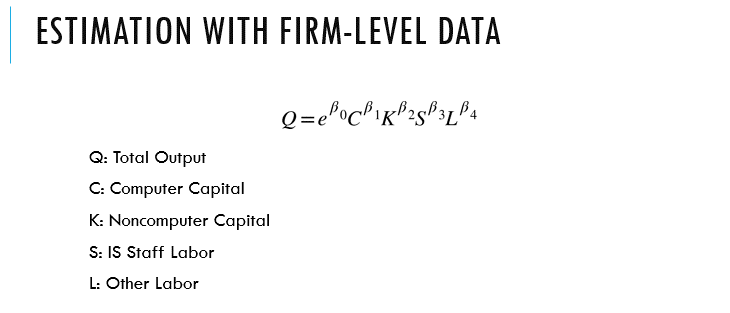
\includegraphics[width=\linewidth]{firmLevelData}

~\\

\textbf{Insights:} Brynjolfsson and Hitt (Management Science, 1996)
\begin{itemize}
\item An additional dollar of computer capital stock is associated with an increase in output of 81 cents per year on the margin An additional dollar spent was associated with a marginal increase in output of \$2.62
\end{itemize}

\vfill\null
\columnbreak

\section{2. Digital Economy and New IT}
\subsection{McKinsey View on 'New' IT}
\begin{itemize}
\item Numerous industries being `reimagined' through IT: To prevent a competitor from re-imagining your product as discontinued or re-imagining your company into liquidation, IT could well be an essential consideration in strategy formulation and execution, and a key area for investment.
\item `Old IT': Addressed labor automation, individual worker productivity, and non-human scale computing;
\item `New IT': Focus on digital products and services, team productivity, and business model transformation.
\item Benefits from old IT have reached a point of diminishing returns; new IT can be a source of competitive differentiation and dramatic wealth creation.
\item \textbf{Business Model Transformation} as a major use of IT, five major levers: Production and operations optimization, Eliminating intermediaries (bypassing middleman), New Monetization models (Amazon Web Services, SaaS etc.), Shaping customer preferences (leveraging big data), Transforming underserved markets (Long Tail phenomenon).
\end{itemize}

\subsection{Traditional Supply Chain Issues}
\begin{itemize}
\item Lack of Coordination between stages in the supply chain where objectives of different stages conflict or information moving between stages is distorted.
\item \textbf{Bullwhip Effect:} Fluctuations in order increases as they move up the supply chain from retailers to wholesalers to manufacturers to suppliers. Distorted demand information, where different stages have different estimates of what demand looks like, amplified variation in demand. Higher safety inventory usually required.
\item Information Processing Obstacles: Forecasting demand based on orders, not customer demand. Lack of information sharing. To overcome tradeoff, we trade responsiveness for cost and vice versa.
\end{itemize}

\subsection{Just-In-Time Production Methods}
\begin{itemize}
\item Tesla Motors has been using Just-In-Time (JIT) production methods to keep costs low since its founding in 2003. (JIT Benefits + Challenges) Tesla is experimenting with lean manufacturing principles in its production processes.
\item JIT is a production strategy that seeks to minimize waste and maximize efficiency by only producing what is needed, when it is needed. This approach requires close coordination between all parts of the production process, from suppliers to assembly line workers.
\item There are some chalenges associated with JIT, such as the need for tight coordination and the potential for disruptions to the production process. However, Tesla has shown that JIT can be an effective production strategy for a high-tech manufacturing company.
\end{itemize}

\subsection{Digital Economy}
\begin{itemize}
\item \textbf{A Digital Economy} takes advantage of the latest technology to digitalise processes and drive business growth. With digital economy, most of economic activities such as production, distribution, and consumption of goods and services are digitalized.
\item Digital technologies reduce the cost of storage, computation, and transmission of data. Therefore, digital economics explores how standard economic models change as certain costs fall substantially and perhaps approach zero.
\item \textbf{IT Capital Investment:} IT Capital Investment by companies has been increasing (in proportion and amount) over the years. IT automate many steps in business processes that were formerly performed manually. IT can enable new innovative business processes by collecting, processing, distributing information in a more efficient and effective way. (e.g., JIT, cross-docking) IT can transform the way the business works and drive new business models.
\end{itemize}
\textbf{Production and Economics of Production: Cost Curves}
\begin{itemize}
\item \textbf{Simple Economics of Production:}
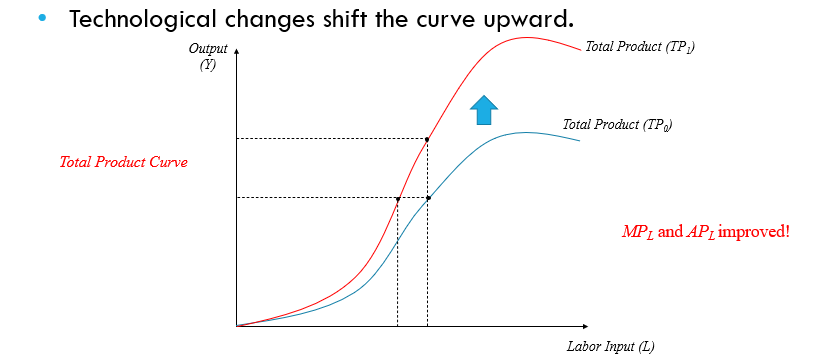
\includegraphics[width=0.7\linewidth]{technologicalChange}
\item \textbf{Economics of Digital Goods:} High fixed costs to produce the first unit, dominated by sunk cost: very high. Marginal production (reproduction) cost : very low. Hence, extensive economies of scale. Can be delivered via the Internet; little distribution cost.
\item DD and SS curve shifts as an impact of technological advances: Demand may shift leftward or rightward depending on the presence of substitutes or complements respectively. Supply increases generally as quality of product and cost of production changes due to technology.
\end{itemize}

\subsection{Disadvantages of Digital Economy}
\begin{itemize}
\item Digital divide: Generally refers to the gap between those who use or have access to telecommunications and information technologies including hardware, internet access, and literacy in using both effectively and those who do not.
\item Cybercrime and Privacy Breaches, Bad ideas spread quickly (e.g., fake news, racism, etc.), Pervasive Advertisement exposure (due to New business model), More monopolistic players (e.g., Google), Addictive nature of technology (Mental health and well-being concerns)
\end{itemize}

\textbf{Summary (of digital technology on businesses)}
\begin{itemize}
\item Digital technology enables economic activities such as production, distribution, and consumption of goods and services are conducted in a more efficient manner.
\item On top of that, digital innovation may lead to a fundamental change through a new economic rule, enhanced collaboration, and innovative business models.
\item However, some other challenges may also arise because of digital technologies
\end{itemize}

\vfill\null
\columnbreak

\section{3. Market Structure}
\begin{itemize}
\item \textbf{Market Power / Dominance} is the ability of a firm or group of firms within a market to profitably charge prices above the competitive level for a sustained period of time. Due to anti consumer and anti competitive issues, huge market power always reduces the economic wealth of society in many ways. (Sherman Antitrust Act US, M\&A regulation, price regulation.)
\item Surge in IT investment by firms from 1995: Internet and enterprise IT accelerated competition within traditional industries. Processes were digitalized through enterprise IT systems. Innovators dominate the market with better ways of doing things. Rivals recapture market shares by roling out further process innovations. Results in increased concentration, turbulence and performance spread.
\subsection{Market Structures (basic economics)}
\item \textbf{Perfect Competition}: Many buyers and sellers with small size, Homogeneous product (little differentiation), Perfect information for buyers and sellers, No transaction/switching costs in market, Free market entry and exit, Equal access to technologies, Company as a price taker. Equilibrium = Normal Profits
\item \textbf{Monopolistic Power}: A monopoly is a company that has "monopoly power" in the market for a particular good or service. The existence of a monopoly relies on the nature of its business. It is often one that displays one or several of the following qualities: Needs to operate under large economies of scale, Requires huge capital, No substitute, Government mandate ensuring its sole existence, Technological superiority and control resources. Disadvantages of a monopoly: Price fixing, declining product quality, loss of innovation, inflation.
\\ Arguments for a `Creative Monopoly': Some advantages of monopoly may include: Economies of scale, Stability of prices, R\&D spending.
\item \textbf{Oligopoly:}: An oligopoly consists of a select few companies that combined exert significant influence over a market or sector. Firms in this case either compete with another to collaborate together (collusion). They use their market influence to set the prices and in turn maximize their profits. Therefore, the consumers become the price takers. In an oligopoly, there are various barriers to entry in the market, and new firms find it difficult to establish themselves. Most countries have laws outlawing such anti-competitive behaviors. Think FAANG or MANGA.
\end{itemize}


\subsection{Porter's Five Forces Framework}
Five forces that determine the competitive intensity and therefore attractiveness of a market.
\begin{itemize}
\item A useful tool (i) to understand the attractiveness of an industry and (ii) to systematically analyze the external environment surrounding a firm. Overall industry attractiveness does not imply that every firm in the industry will return the same profitability. Competitive advantage of a firm is achieved by enhancing a firm’s ability to combat the 5 forces.
\item \textbf{Force 1: Bargining Power of Supplier}: Supplier power is high when there is domination of supply by a few companies. (Examples: Crude Oil Suppliers (OPEC)), product is unique or at least differentiated, has built up switching costs (Examples: Database (Oracle), MS Windows, Cell phone services), provides benefits through geographic proximity to its customers. ( Examples: Convenient stores), poses a definite threat to forward integrate into its customers’ business. (Examples: Movie studios that also own a chain of theatres).
\item \textbf{Force 2: Bargining Power of Buyer/Consumer}: Buyer’s bargaining power is high when it has large, concentrated buying power that enables it to gain volume discounts and/or special terms or services (Examples: organizational buyers like Wal-Mart, Costco, Safeway), what it is buying is standard or undifferentiated and there are multiple alternative sources, product is unimportant to the quality of the buyers’ products or services. (Examples: buyers of commodity type of products), has a strong potential to backward integration. (Examples: airline companies that also own aircraft maintenance and in-flight catering businesses).
\item \textbf{Force 3: Substitute Products or Services}: Substitutes: a product or service in another industry which can fulfill the same needs. Threat of substitute products or services is high when  Relative price performance of substitutes is high, Switching cost to new products is low, Buyer propensity to substitutes is large.
\item \textbf{Force 4: Threat of Potential New Entrants}: The threat of new entrants is high when it is easy for new competitors to enter a market, low when there are significant entry barriers to entering a market. Common sources of the entry barrier include: Regulation, Patents and proprietary knowledge, Economies of scale: Newcomer’s cost per product is higher, Capital requirement, Difficulty in brand switching, Difficulty in accessing distribution channel.
\item \textbf{Force 5: Rivalry among Existing Competitors}: Intra-industry rivalry is intense when Competitors are numerous or roughly equal in size and power, Industry growth is slow, precipitating fights for market share, and the product lacks differentiation or switching costs.
\end{itemize}

\subsection{Internet's Impact on Industries \& Forces}
\begin{itemize}
\item \textbf{Impact on Industries}: High Industry concentration, High Turbulence (the top-selling company one year may not dominate next year. Today’s \#10 company, for instance, might jump to \#1 the following year.) Large and Growing Performance Spread: Increasing spread in gross profit margin.
\item \textbf{Impact on Market Structures}: `Easier to become a monopoly in Digital Economy': Network Effects (“Winner takes all” phenomenon) (value of service depends on number of users), High switching cost, Economies of scale, High initial fixed cost and low marginal cost of production. Convergence of digital services (Blending of previously separate technologies, processes, and data to create new combinations of products, services, and experiences that reshape industry structures It is much easier to create new services by combining multiple services), AI \& Data analytics, Hard to regulate.
\item \textbf{Digital Business vs. Traditional Market:} Market definition is complicated by zero-pricing for the use of many digital platforms and the subsequent harvesting of consumer data. For many digital platforms, consumers forfeit their data (rather than money) in exchange for the services they receive (e.g., Google, YouTube, etc).
\item \textbf{Impact on Competitive Dynamic of each Force}:  Adds entry barriers to new entrances, enables foothold in rivalry among existing competitors, adds to switching cost reducing buyer power. (e.g. American Airlines (SABRE) Reservation system, Display bias, 80\% of reservation conducted on first page, Information over competitor, Co-host program with partner airlines bargining power, new business creation, enabled AA to expand busines scope into information business.)
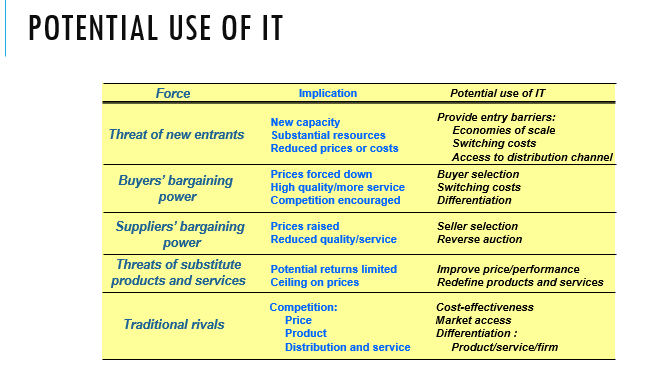
\includegraphics[width = \linewidth]{portersIT}
\\ ~\\
\textbf{Internet's Impact on Five Forces:}
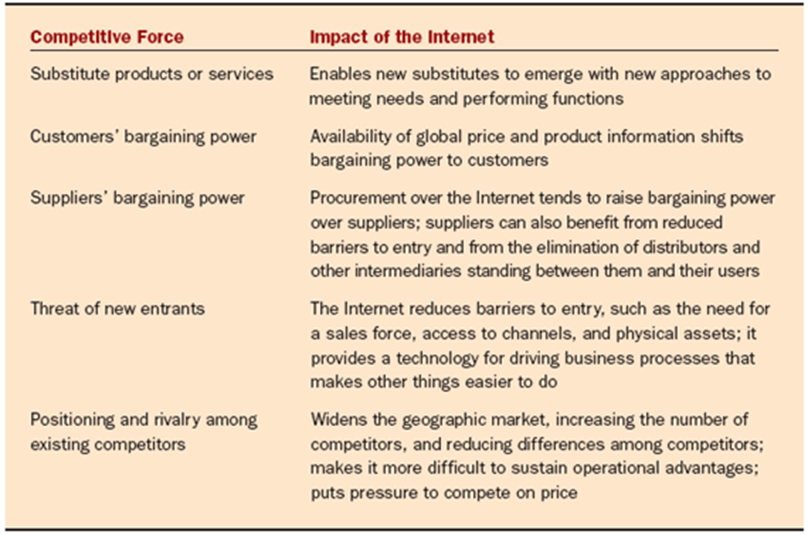
\includegraphics[width = \linewidth]{portersInternet}
\end{itemize}

\vfill\null
\columnbreak

\section{4. Pricing, Bundling and Subscription Model}
Pricing: (Most important determinant of consumption of goods/services. Aim for Profit maximizing price)
\subsection{Economic Value to Customer}
\begin{itemize}
\item \textbf{EVC:} Measure of how much value an individual customer, or customer segment, gets from using a company’s products or services: It includes both tangible and intangible benefits. Underlying economic theory: Customer will buy a certain product only if its utility to them outweights that of the closest alternatve (total satisfaction or benefit).
\centerline{\textbf{EVC = Reference Value $+$ Differentiation Value}}
\item Reference Value: Price of what customer views as the best substitute
\item Differentiation Value: Value of differentiating attributes over the best substitute.
\item \textbf{Sources of Customer Value}: Benefits or costs associated with availability, convenience, functionality, relationship, brand image. Example: Starbucks differentiation value through branding. 
\item  \textbf{Application of EVC: } EVC leads to maximum willingness to pay (WTP). EVC is determined by reference and differentiation value, consumer choices is determined by net value. Can derive demand curve based on understanding of customer value, and obtain profit maximizing price level.
\item \textbf{Developing Pricing Strategy}: In reality, customers are very different (heterogenous) in terms of taste and WTP. Must assess value customers place on product and WTP, through market research, customer contact, etc or qualitiative or quantitative methods.
\end{itemize}

\subsection{Price Discrimination}
Price Discrimination: Charging customers different prices for the same product. 
\begin{itemize}
\item \textbf{First degree (Perfect) price discrimination}: Individual pricing (personalized pricing): Becoming easier, but may face some controversies and resistance (Amazon price-testing program raises anger, cola vending machine price related to temperature, singer album price increase after death)
\item \textbf{Second degree price discrimination}: (versioning or menu pricing): Create different products for the purpose of price differentiation (Easily done for Software → Full features and value-subtracted to target different segments, e.g. math software pro vs student version, quicken software). Versioning: firm engages in differential pricing by offering different versions of a product, e.g. IBM spent additional money to insert a chip to slow down one of its printers → Marginal cost is incurred! However, for digital products, creation of different versions is so easy for digital goods/services! (because MC=0).
\item \textbf{Third degree price discrimination}: Group pricing based on segmentation, when a company charges a different price to different consumer groups. Firms try to generate sales by identifying different market segments, such as domestic and industrial users, with different price elasticities. (e.g. Student or Senior Price) Identifying such segments and implementation of differential prices have become much easier with digital technologies! Digital technologies including AI-based methods enable such price discrimination at more affordable costs
\end{itemize}

\subsubsection{Using Big Data to adopt Price Discrimination:}
3Vs: Volume, Velocity and Variety of Data.
\begin{itemize}
\item \textbf{Volume}: A large amount of data, which makes the conventional approaches and algorithms inefficient and less applicable.
\item \textbf{Velocity}: Real-time or nearly real-time information makes it possible for a company to be much more agile than its competitors.
\item \textbf{Variety}: Many sources, different data formats, highly unstructured (Messages, images, videos, readings from sensors, GPS signals from cell phones, etc)
\item These data help firms better understand customers and develop accurate and more effective pricing strategies. How? → Price discrimination
\\ ~\\
\item \textbf{Types of Data categorised via 3Vs}
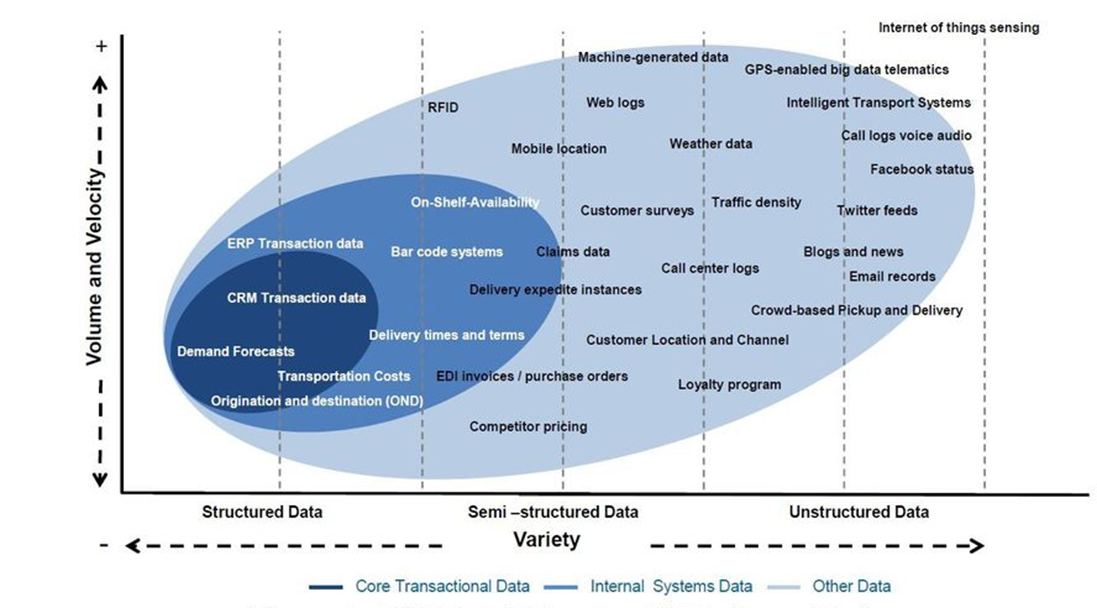
\includegraphics[width = \linewidth]{bigData3V}
\end{itemize}


\subsection{Capturing Consumer Information and using it with AI }
\begin{itemize}
\item \textbf{Marketing Funnel}: A series of stages to guide prospects through the customer journey. Crucially, what data do they need at each stage?
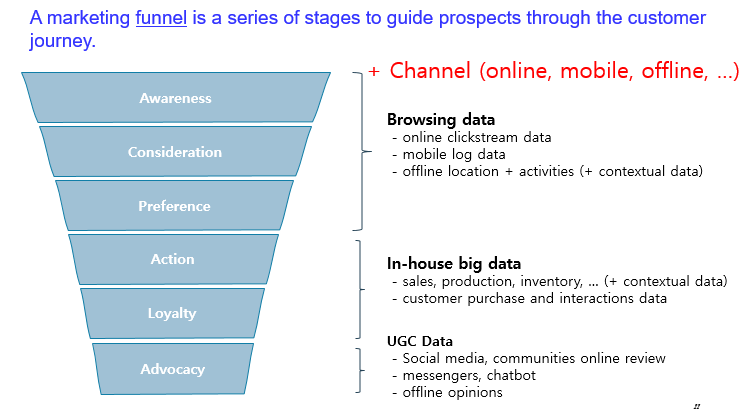
\includegraphics[width = \linewidth]{marketingFunnel}
\item \textbf{User Generated Content UGC}:UGC is at least as valuable as a source of customer needs for product development, likely more valuable, compared with conventional methods. Machine-learning methods improve efficiency of identifying customer needs from UGC (unique customer needs per unit of professional services cost). (See potential system architecture for identifying customer needs from UGC.) E.g. Study Timoshenko et al (2019): UGC captures vast majority of customer needs (97\%), opportunities for prodct improvement (92\%) and hidden opportunities (92\%)for oral-care products.
\end{itemize}

\subsection{Bundling: (Combining products and pricing)}
\begin{itemize}
\item Can be considered a form of (second degree) price discrimination, Discriminate by quantity and features. 
\item Bundling can be also easily done through digital technologies! (low menu cost, marginal cost, cost of implementation, etc)
\end{itemize}

\subsection{Subscription Model: (Type of PD and bundling)}
\begin{itemize}
\item Businesses may benefit because of predictable and constant revenue stream from subscribed individuals.
\item Many digital services are offering a subscription-based pricing.
\end{itemize}

\textbf{Summary}: Consumers are heterogenous, making different pricing strategies more effective. Digital technologies have enabled firms to extract more surplus from consumers because it is now easier to estimate their WTP and implement different pricing schemes for price discrimination (low marginal cost of production, lower menu cost, low cost of implementation).


\vfill\null
\columnbreak

\section{5. Network Effects }

\subsection{Externalities}
\begin{itemize}
\item \textbf{ An externality}: an indirect cost or benefit to an uninvolved third party that arises as an effect of another party's (or parties') activity. That is, an externality is an event the occurs as a byproduct of another event occurring. Can be positive or negative and can stem from either the production or consumption of a good or service.
\item Example: R\&D of a company can be a positive externality. R\&D increases the private profits of a company but also has the added benefit of increasing the general level of knowledge within a society. Pollution caused by commuting to work or a chemical spill caused by improperly stored waste are examples of negative externalities.
\end{itemize}
\subsection{Network Effects}
\begin{itemize}
\item\textbf{Network Effect} is the phenomenon by which the value or utility a user derives from a good or service depends on the number of users in general and user connection in particular, in the product/service network.
\item Network effects are typically positive (i.e., positive externalities), resulting in a given user deriving more value from a product as more users join the same network.
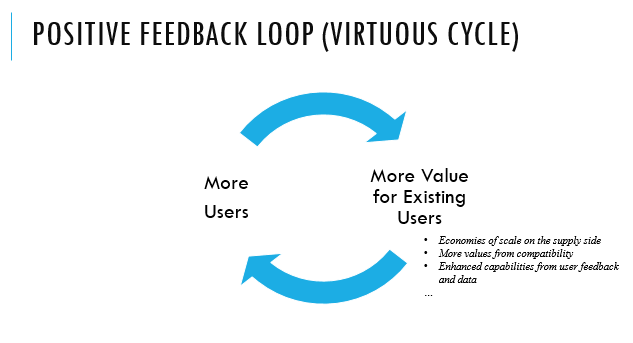
\includegraphics[width=\linewidth]{positiveFeedbackLoop}
\item Congestion is a negative network effect whereby too many users can slow a network down, reducing its utility and frustrating network members.
\item \textbf{Metcalfe's law} states that the value of a telecommunications network is proportional to the square of the number of connected users of the system. (1993) Assumes all nodes have equal benefits and are all connected, but many social networks don’t exactly match Metcalfe law because some new nodes don’t create connections with all existing nodes. Also, In social networks, new entrants that join later and have different interests and expertise may not create connections with existing users. This decreases benefit of each additional user, making the overall network less efficient if costs per users are fixed.
\end{itemize}
\subsection{Network Effects in Digital Economy}
\begin{itemize}
\item Network effects have become a defining property of the digital economy, since the business model of many digital services is based on matchmaking (e.g., Uber, Airbnb, Gig economy platforms) and mediation between users (e.g., YouTube, Facebook).
\item The positive feedback is not totally new but is a \textbf{more potent force} in the digital economy than ever before, often leading to a \textbf{winner-takes-all market}.
\item \textbf{AI and Positive Feedback (of usage)}: Good data can lead to a positive feedback loop with advanced decision recommendation and analytics today. It would be more critical in the age of AI. However, having good data for training of algorithms may be challenging in certain contexts.
\end{itemize}
\subsection{Impact of Network Effects on Pricing: Freemium Models}
\begin{itemize}
\item \textbf{Price Differently}: As a business grows due to the network effect, it often makes sense to increase prices as demand for the product grows. However, starting at a lower price (or in some cases, giving the product away for free, as mentioned above) and then increasing the price of the product as the network effect occurs will result in a larger user base.
\item \textbf{Freemium}: business model in which a company offers basic or limited features to users at no cost and then charges a premium for supplemental or advanced features. Freemium models are especially popular among software applications and internet-based businesses (partly because MC=0).
\end{itemize}
\subsection{Two-sided Network (Platforms) Effects}
\begin{itemize}
\item \textbf{Two-sided networks}: Products and services that bring together groups of users in two-sided networks are platforms. Examples: Operating Systems, B2B Exchanges, Online recruitment.
\item Platforms provide infrastructure and rules to facilitate the two groups’ transactions and can take many forms. When successful, the platforms catalyze a virtuous cycle; More demand from one side spurs more from the other. (e.g. Ebay)
\end{itemize}
\subsection{Effective Strategies \& Considerations in Presence of Two-Sided Network Effects}
In the e-commerce environments, you may have to deal with the two-sided network effects. It is tricky to manage platforms successfully
\begin{itemize}
\item \textbf{Disruptive Force}: Disrupting Existing Networks (Zoom vs Skype): Zoom is actually built on allowing “frictionless” communication between users the service is not meant to only work for those in its network, where zoom user can video call anyone by sending link, where recipient does not even need to have a Zoom account.
\item \textbf{Pricing}: Subsidize one user group (quality and price sensitive users) while charging the other a premium for access to the subsidized group (E.g., Adobe’s Acrobat PDF maker). Secure important users’ exclusive participation in your platform by providing incentives (E.g., government, LV in the airport).
\item \textbf{Coping with Winner-Takes-All Competition}: Decide whether the two-sided market you’re eyeing will eventually be served by a single platform. If yes, it is risky to fight for proprietary control (E.g., Video players, App Store).
\item \textbf{Consumer Protection and Legal Issues}: Examples: Counterfeit products on e-commerce websites, Legal responsibilities for platform “gig” workers, Consumer privacy and data breaches, can affect company stock prices.

\end{itemize}•



\vfill\null
\columnbreak

\section{6. Lock-in and Switching Costs}
\subsection{Definition of Lock-In}
\subsection{Definition of Switching Cost}
\subsection{Lock-in and Market Failure}
\subsection{Lock-in as a Strategy of Digital Business}
\subsection{Classification of Lock-in}
\subsection{CRM: Customer Relation Management}
\subsection{Operational Vs. Analytical CRM}

\vfill\null
\columnbreak

\section{7. Free Riding and Contribution}
\subsection{Private vs. Public Goods}
\subsection{Public Goods in the Digital Economy - Undercontribution (Free-Rider Problem)}
\subsection{Motivating Participation \& Solutions}
\subsection{Tragedy of the Commons}
\subsection{Sharing Economy}

\vfill\null
\columnbreak

\section{8. Information Asymmetry / Transaction Cost Economics}
\subsection{Information Asymmetry: \& Risk in Economics}
\subsection{Risk \& Uncertainty In Economics}
\subsection{Risk Aversion \& Product Quality}
\subsection{Asymmetric Information}
\subsection{Adverse Selection: Market Failure}
\subsection{Quality Uncertainty in Digital Businesses}
\subsection{Operational Vs. Analytical CRM}
\subsection{Adverse Selection: Market Failure}
\subsection{Solutions to Adverse Selection (Signal \& Screen}
\subsection{Moral Hazard}
\subsection{Risk Aversion \& Decisions (Use of analytics to infer risk)}


\vfill\null
\columnbreak

\section{9.  Search Cost \& Transaction Cost}
\subsection{IT Services Market \& Outsourcing }
\subsection{Transaction Cost Economics (TCE)}
\subsection{Platforms in TCE}
\subsection{“Long Tail Phenomenon”}
\subsection{Search Cost }


\vfill\null
\columnbreak

\section{10: Behavioral Economics}
\begin{itemize}
\item \textbf{Behavioral Economics} combines elements of economics and psychology to understand how and why people behave the way they do in the real world. Differs from neoclassical economics, which assumes that most people have well-defined preferences and make well-informed, self-interested decisions based on those preferences. 
\item \textbf{[Grounded in] Empirical observations of human behavior}, which have demonstrated that people do not always make what neoclassical economists consider the “rational” or “optimal” decision, even if they have the information and the tools available to do so. (People are sometimes irrational)
\end{itemize}
\subsection{Nudging}
\begin{itemize}
\item \textbf{Nudge}: Thaler and Sunstein (2008, p. 6), is any aspect of the choice architecture that alters people's behavior in a predictable way without forbidding any options or significantly changing their economic incentives.
\item Examples: Placing healthier food choices at eye level or near cash register in schools, compared to banning junk food. Thaler: Changing test scores to be out of 137 instead of 100. Study that yielded fuel savings in flights.
\end{itemize}
\subsection{Loss Aversion}
\begin{itemize}
\item In general, if dealing with loss aversion, people are more willing to take risk (to avoid loss). With “prospect theory,” Tversky and Kahneman demonstrated that framing and loss aversion influence the choices people make. 
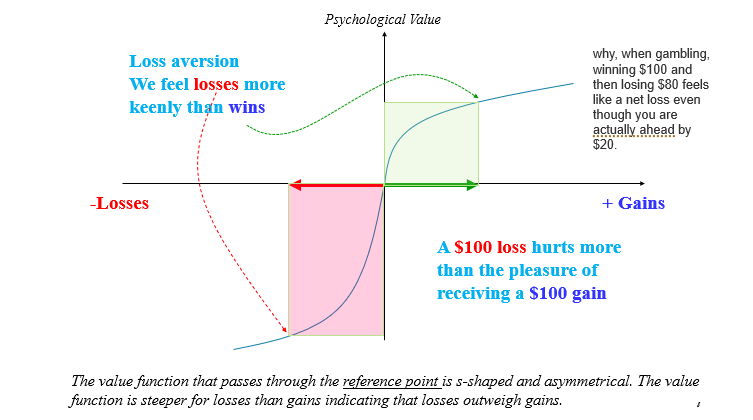
\includegraphics[width =\linewidth]{lossAversion}
\end{itemize}
\subsection{Confirmation Bias}
\begin{itemize}
\item Refers to people's tendency to process information by looking for, or interpreting, information that is consistent with their existing beliefs.This biased approach to decision making is largely unintentional, and it results in a person ignoring information that is inconsistent with their beliefs.
\item In social media, confirmation bias is amplified by the use of filter bubbles, or "algorithmic editing", which display to individuals only information they are likely to agree with, while excluding opposing views.\item A filter bubble is a state of intellectual isolation that can result from personalized searches, where a website algorithm selectively curates what information a user would like to see based on information about the user, such as location, past click-behavior, and search history.
\end{itemize}
\subsection{Sunk Cost Fallacy}
\begin{itemize}
\item \textbf{Sunk Cost}: Refers to money that has already been spent and cannot be recovered.
\item The sunk cost fallacy refers to a greater tendency to continue an endeavor once an investment in money, effort, or time has been made. This is like "throwing good money after bad“.
\item Even though economists argue that sunk costs are not at all relevant to future rational decision-making, people in everyday life often take previous expenditures in situations, such as repairing a car and gambling loss into their future decisions regarding those properties.
\end{itemize}
\subsection{Digital Nudging}
\begin{itemize}
\item A subtle form of using design, information and interaction elements to guide user behavior in digital environments, without restricting the individual's freedom of choice.
\item The use of digital nudges has become prevalent and is widely adopted in various domains. With digital technologies, it is much easier to implement such “nudges” and influence user behaviors (recall the “zero marginal cost” in digital economy) In addition, we spent more and more time with digital technologies.
\item Re-analysis of meta-analysis reveals no evidence for nudging once accounting for publication bias: A 2022 meta-analysis that nudging was an effective tool for behavior modification. However, the authors also found significant publication bias toward positive results in the literature, with a sensitivity analysis revealing a miniscule effect size in the case of severe publication bias.
\item In reality, designing appropriate nudges that work consistently and reliability is very challenging.
\end{itemize}
\subsection{Field Experiment (AB Test)}
\begin{itemize}
\item A/B testing, also known as split testing, refers to a randomized experimentation process wherein two or more versions of a variable (web page, page element, etc.) are shown to different segments of website visitors at the same time to determine which version leaves the maximum impact and drives business metrics.
\item \textbf{p-Hacking}: defined as “try[ing] out several statistical analyses and/or data eligibility specifications and then selectively report[ing] those that produce significant results. They may stop their experiments based on the p-value of the treatment effect. Study found false discovery rate (FDR) ranges between 28\% and 37\% for tests conducted at 10\% significance level (less robust).
\end{itemize}

\vfill\null
\columnbreak


\section{11: Economic Impacts of AI}
\subsection{Artificial Intelligence}
\begin{itemize}
\item Broadly speaking, AI refers to the ability of a digital computer or computer-controlled robot to perform tasks commonly associated with intelligent beings.
\item Characterizing AI precisely is also difficult because the definition tends to change depending on the specific context of research and application. AI is widely used to analyze big data, identify patterns, and predict outcomes
\item \textbf{Turing Test} to define AI: If a computer can talk like a human and cannot be told apart, then the computer can think like a human. ChatGPT is known to have passed the Turing test.
\end{itemize}
\subsection{Labor Substitution by AI}
\begin{itemize}
\item Who will be replaced? Who will do a better job does not necessarily mean the actual or immediate replacement. That is, it is not matter of efficiency or technology. Additionally, income or social status does not necessarily mean a lower chance of replacement either.
\item \textbf{Investment and Employment}: Impact on employment not obvious yet. Data from robots imported by Canadian firms by the Canadian Border Services Agency (CBSA) from 1996 to 2017, found that: Robots may directly reduce need to monitor workers when robots reduce human errors in production process. Although the total number of nonmanagerial employees increases with robot adoption, robot investments predict decreases in employment of middle-skilled workers and increases in employment of low- and high-skilled labor
\item “From Agriculture to Art — the A.I. Wave Sweeps In,” NY Times, (2018): Artificial intelligence is a technology of low-cost prediction and discovery. It exploits the new resource of the digital age —vast amounts of data —to identify patterns and make predictions. Much of what A.I. does today can be thought of as a prediction.
\end{itemize}
\subsection{Economic Impact at Different Levels}
\begin{itemize}
\item In general, the impact of digital technologies we have discussed will be amplified. However, we will have to deal with many new issues. It is very difficult to predict what is going to happen at this point.
\item \textbf{Country}: Digital divide will be reinforced, The gap between leading countries and developing countries will be widened. Retraining will become a critical issue. New business models also possible.
\item \textbf{Company}: Performance gap will be widened between front-runners and non-adopters, Use AI for labor augmentation or substitution of production factors
\item \textbf{Individual / Workers}: More jobs will be replaced or augmented with AI.
\end{itemize}
\subsection{Adoption of AI by Companies \& Issues}
\begin{itemize}
\item On top of technological issues, companies need to address more issues to adopt AI in businesses: Black box problem, Consumer reaction, Regulation and Ethical issues.
\item \textbf{Black Box Problem}: (Lack of explanability) As models become more sophisticated they begin to evolve from simple linear models to non-linear combinations, occasionally of other more complicated models. This is known as the “Black Box Problem” in machine learning. This significantly limits the applicability of AI models especially when the failure in systems leads to a serious problem (e.g., threatening human lives)
\item \textbf{Consumer Reactions}: Consumers may react either positively or negatively to Ais depending on the different contexts. Anthropomorphism is one of the important elements to be considered for robots and AI. It is generally described as “the attribution of human-like qualities to nonhuman entities such as machines, animals, and other objects: Uncanny Valley: 1970s, Professor Masahiro Mori, observation that as robots appear more humanlike, they become more appealing - but only up to a certain point. Upon reaching the uncanny valley, our affinity descends into a feeling of strangeness, unease, and freakiness. Justifies people’s negative reaction to certain lifelike robots.
\item Results suggest that undisclosed chatbots are as effective as proficient workers and four times more than inexperienced in engendering customer purchases. However, disclosure of bot identity before the convo reduces purchase rates by more than 79.7\%.
\end{itemize}

\vfill\null
\columnbreak


\section{12: Risks and Regulation of AI}










\end{multicols*}
\end{document}
